\section{tasks::check\-Integrity Class Reference}
\label{classtasks_1_1checkIntegrity}\index{tasks::checkIntegrity@{tasks::checkIntegrity}}
Inheritance diagram for tasks::check\-Integrity::\begin{figure}[H]
\begin{center}
\leavevmode
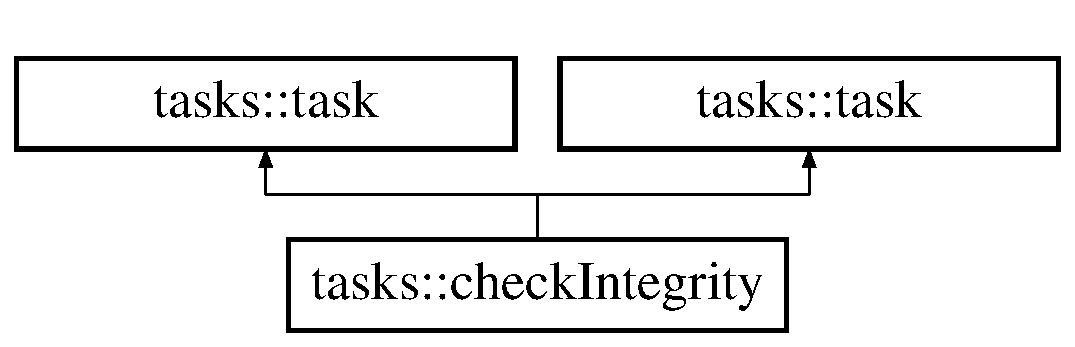
\includegraphics[height=2cm]{classtasks_1_1checkIntegrity}
\end{center}
\end{figure}
\subsection*{Public Member Functions}
\begin{CompactItemize}
\item 
def \textbf{run}\label{classtasks_1_1checkIntegrity_d99d0317b8fed824abc8e321d80d6e1f}

\item 
def \textbf{run}\label{classtasks_1_1checkIntegrity_d99d0317b8fed824abc8e321d80d6e1f}

\end{CompactItemize}
\subsection*{Static Public Attributes}
\begin{CompactItemize}
\item 
string \textbf{name} = '{\bfcheck\-Integrity}'\label{classtasks_1_1checkIntegrity_9fdf082ac655a342a8dc25f091b03369}

\item 
string \textbf{button\-Text} = 'Check Integrity'\label{classtasks_1_1checkIntegrity_a05a9c7fa45d9970c65cad1f754a299f}

\end{CompactItemize}


\subsection{Detailed Description}


\footnotesize\begin{verbatim}Check image Integrity: For the moment, compute mode and check if is under/over
a defined mode value. Bad images will be moved to a BADIMAGES directory

\end{verbatim}
\normalsize
 



The documentation for this class was generated from the following files:\begin{CompactItemize}
\item 
old/PANICtool-1.0/tasks.py\item 
old/tasks.py\end{CompactItemize}
